    \documentclass[12pt,a4paper,oneside]{report}

\usepackage[left=1.25in,right=1in,top=1in,bottom=1in]{geometry}
\usepackage{titlesec}
\usepackage{setspace}
\usepackage{times}
\usepackage{fancyhdr}
\usepackage{graphicx}
\usepackage{tabularx}
\usepackage{array}
\usepackage{caption}
\onehalfspacing

\setlength{\headheight}{14pt}
\setlength{\headsep}{25pt}
\setlength{\footskip}{25pt}

\titleformat{\chapter}[display]
  {\normalfont\bfseries\Large\centering} % formatting
  {CHAPTER \thechapter}                  % chapter number
  {10pt}                                 % space between number and title
  {\Large}  
% Adjust chapter spacing
\titlespacing{\chapter}{0pt}{-30pt}{10pt}
% -----------------------------
% Main Header & Footer (For Chapters)
% -----------------------------
\pagestyle{fancy}
\fancyhf{}

\fancyhead[R]{\textit{Short Title}}

\fancyfoot[L]{AY 2026-27}
\fancyfoot[C]{Department of Computer Science and Engineering}
\fancyfoot[R]{Page \thepage}

\renewcommand{\headrulewidth}{0.8pt}
\renewcommand{\footrulewidth}{0.8pt}

% Apply header/footer on chapter starting pages
\fancypagestyle{plain}{
  \fancyhf{}
  \fancyhead[R]{\textit{Short Title}}
  \fancyfoot[L]{AY 2026-27}
  \fancyfoot[C]{Department of Computer Science and Engineering}
  \fancyfoot[R]{Page \thepage}
  \renewcommand{\headrulewidth}{0.8pt}
  \renewcommand{\footrulewidth}{0.8pt}
}

% -----------------------------
% Front Matter Style (NO header/footer)
% -----------------------------
\fancypagestyle{frontmatter}{
  \fancyhf{}
  \fancyfoot[C]{\thepage}            % Roman page number centered
  \renewcommand{\headrulewidth}{0pt}
  \renewcommand{\footrulewidth}{0pt}
}


% =============================
% DOCUMENT STARTS
% =============================
\begin{document}

% =============================
% FRONT MATTER (Roman numbering)
% =============================
 \fancypagestyle{plain}{
  \fancyhf{}
  \fancyfoot[C]{\thepage}
  \renewcommand{\headrulewidth}{0pt}
  \renewcommand{\footrulewidth}{0pt}
}
\pagenumbering{roman}
\setcounter{page}{1}
\pagestyle{frontmatter}


% -------- Acknowledgement --------
\chapter*{\centering\Large\bfseries ACKNOWLEDGEMENT}
\addcontentsline{toc}{chapter}{ACKNOWLEDGEMENT}
\pagestyle{frontmatter}
  \begin{spacing}{1.75}

If words are considered tokens of acknowledgement, then they play a heraldic role, expressing our gratitude.

With proud gratitude, we thank God Almighty for all the blessings showered on us and for completing our project successfully.

We extend our heartfelt gratitude to the Management of \textbf{A. J. Institute of Engineering and Technology}, a unit of \textbf{Laxmi Memorial Education Trust}, for their unwavering support throughout our project journey.

We owe our gratitude to The Principal, \textbf{Dr. Ashok Kumar T} for his whole-hearted support and for his kind permission to undertake the project.

We are indebted to the Dean Academics, \textbf{Mr. Mahabaleshwarappa P}, for his guidance and invaluable suggestions, steered us towards a greater insight and understanding.

We wish to express our deepest gratitude to \textbf{Dr.Chanchal Antony}, Head of Department, Computer Science and Engineering(Artificial Intelligence \& Machine Learning), AJIET, for his profound alacrity in our project and his valuable suggestions. 

We wish to enunciate our special thanks to our paradigmatic and relevant \textbf{Project coordinator},\textbf{Dr.Vineetha Pais},Associate Professor,and the internal guide \textbf{Dr.Pradeep Udupa}, Associate Professor,Department of Computer Science and Engineering(Artificial Intelligence \& Machine Learning),AJIET,who gave us throughout our project period with their valuable suggestions and for devoting their precious time in making this project a success.

Finally, we offer our sincere thanks to our family members and friends for their valuable suggestions,encouragement,and unwavering support.

\begin{flushright}
   \begin{tabular}{cc}
       
      \hspace{-15em}   \textbf{Name}  \hspace{2em}    & \textbf{USN} \\
     
\hspace{-15em} \textbf{ADITHYA JAYAN }  \hspace{2em}  & \textbf{4JK23CI005} \\
 \hspace{-15em}    \textbf{ADITHYAN M} \hspace{2em}   & \textbf{4JK23CI006 }\\
\hspace{-15em}       \textbf{MAZIN HAMEED}  \hspace{2em}  & \textbf{4JK23CI029} \\
\hspace{-15em}     \textbf{ SHAAZ OMAR} \hspace{2em}   & \textbf{4JK23CI049} \\
       
    \end{tabular}

\end{flushright}
  \end{spacing}
% -------- Abstract --------
\chapter*{\centering\Large\bfseries ABSTRACT}
\addcontentsline{toc}{chapter}{ABSTRACT}
\pagestyle{frontmatter}
Legal and administrative documents often contain complex terminology, lengthy clauses, and formal language that can be difficult for non-expert users to understand. **LexiClear** is an AI-assisted document-understanding system designed to make such information more accessible through automated document processing, semantic retrieval, and natural-language interaction. The system accepts legal and administrative PDF documents, including scanned documents, and uses direct text extraction or Optical Character Recognition (OCR) to obtain machine-readable content. The extracted text is preprocessed, divided into meaningful chunks, converted into semantic embeddings, and stored for efficient retrieval. LexiClear applies Retrieval-Augmented Generation (RAG) to retrieve relevant document content and generate responses grounded in the uploaded document. It provides structured analysis covering aspects such as summary, risks, obligations, rights, clauses, and required actions where applicable, while the **Ask LexiClear** interface enables users to ask document-specific questions. Jurisdiction grounding is incorporated to provide additional contextual information where configured. To improve accessibility, the system supports **English, Hindi, and Kannada** output along with text-to-speech functionality through Listen and Stop controls. The system is implemented using a React-based frontend with Vite and a FastAPI backend, integrating document processing, retrieval, generation, translation, and speech capabilities into a unified workflow. Functional testing demonstrates the operation of document upload and processing, structured analysis, question answering, multilingual output, jurisdiction grounding, and speech generation. LexiClear is intended as an AI-assisted comprehension and information-access tool that helps users understand complex documents more easily, rather than as a substitute for qualified legal professionals or authoritative legal advice.


\clearpage




% -------- Table of Contents --------
\renewcommand{\contentsname}{\centering\Large\bfseries CONTENTS}
\tableofcontents
\pagestyle{frontmatter}
\clearpage

% -------- List of Figures --------
\renewcommand{\listfigurename}{\centering\Large\bfseries List of Figures}
\addcontentsline{toc}{chapter}{List of Figures}
\listoffigures
\pagestyle{frontmatter}
\clearpage

% -------- List of Tables --------
\renewcommand{\listtablename}{\centering\Large\bfseries List of Tables}
\addcontentsline{toc}{chapter}{List of Tables}
\pagestyle{frontmatter}

\listoftables
\clearpage

% =============================
% MAIN MATTER (Arabic numbering)
% =============================
\fancypagestyle{plain}{
  \fancyhf{}
  \fancyhead[R]{\textit{LexiClear: Making Legal Language Accessible Through AI}}
  \fancyfoot[L]{AY 2026-27}
  \fancyfoot[C]{Dept. of CSE(AIML), AJIET, Mangaluru }
  \fancyfoot[R]{Page \thepage}
  \renewcommand{\headrulewidth}{1.8pt}
  \renewcommand{\footrulewidth}{1.8pt}
}
\pagenumbering{arabic}
\pagestyle{plain}


\chapter{Introduction}

\section{Background and Motivation}

Legal and administrative documents play an important role in everyday personal, professional, financial, and institutional activities. Individuals regularly encounter documents such as rental agreements, employment contracts, insurance policies, loan and financial documents, government notices, organizational policies, service agreements, and other formal records. These documents contain important information regarding rights, responsibilities, obligations, conditions, restrictions, deadlines, penalties, and possible risks. However, the information contained in such documents is often difficult for ordinary users to understand because of formal terminology, lengthy sentences, complex clause structures, cross-references, exceptions, and domain-specific language. As a result, users may understand the general purpose of a document but still have difficulty identifying the specific conditions or obligations that directly affect them. The earlier LexiClear work identified this difficulty as a central motivation for developing an AI-assisted system for making complex legal information more accessible.

\subsection{Challenges in Understanding Legal Documents}

The difficulty becomes more significant when a user needs to locate a particular piece of information quickly. Reading an entire legal or administrative document manually can be time-consuming, particularly when the document contains several pages of detailed clauses. A user may want to know questions such as what obligations are imposed on them, what rights are provided, whether a particular condition exists, what actions are required, or what potential risks should be considered. Conventional document search based only on keywords may not always provide an effective solution because the wording used by the user may differ from the wording used in the document. For example, a user may ask about the consequences of ending an agreement, while the document may describe the same concept using formal terminology related to termination, notice periods, or contractual conditions. Therefore, an effective document-understanding system needs to consider the semantic meaning and context of the user's query rather than depending exclusively on exact keyword matching.

\section{Artificial Intelligence and Natural Language Processing}

Artificial Intelligence (AI) and Natural Language Processing (NLP) provide techniques that can be used to address these challenges. Recent developments in semantic embeddings, vector-based information retrieval, Optical Character Recognition (OCR), and generative language models make it possible to process large amounts of unstructured document content and retrieve information according to its semantic meaning. LexiClear builds upon these technologies to create a document-oriented system in which the uploaded document is converted into machine-readable content, processed into meaningful sections, represented using semantic embeddings, and made available for contextual retrieval. The earlier implementation established the core pipeline involving document processing, text extraction, preprocessing, chunking, embeddings, vector retrieval, and Retrieval-Augmented Generation (RAG).

\section{Document Processing and OCR}

A major requirement of the system is the ability to handle different types of input documents. Legal and administrative information is not always available in digitally selectable form. Some documents are scanned pages or image-based PDFs in which the text cannot be directly extracted using conventional PDF processing methods. To address this limitation, LexiClear supports both direct text extraction and Optical Character Recognition. When machine-readable text is available, the system can extract it directly from the PDF. For scanned or image-based content, OCR is used to convert the visual representation of the document into machine-readable text. The extracted content can then be cleaned, processed, divided into suitable chunks, and prepared for subsequent semantic analysis. This makes the system applicable to a wider range of real-world documents rather than being restricted only to digitally generated PDFs.

\section{Semantic Retrieval and RAG}

After extraction, the document content is processed so that relevant information can be retrieved efficiently. The text is divided into meaningful chunks and converted into numerical vector representations using semantic embeddings. These representations allow the system to identify content that is conceptually related to a user's query, even when the exact words used in the query are not present in the document. The resulting vectors can be stored in a vector-based knowledge or retrieval system. When a user asks a question, the question is represented in the same semantic space and the system retrieves document sections that are most relevant to the query. This retrieval mechanism forms an important part of LexiClear because the objective is not simply to generate a fluent response, but to connect the response with information contained in the uploaded document.

\subsection{Retrieval-Augmented Generation}
LexiClear uses Retrieval-Augmented Generation as the primary approach for generating document-grounded explanations. In a conventional generative AI interaction, a language model may generate an answer based largely on information learned during training. Such an approach can be unsuitable for document-specific questions because the response may contain information that is not present in the uploaded document. The RAG approach addresses this issue by retrieving relevant document content before generating the response. The retrieved information is supplied as context to the generation process, allowing the response to remain more closely connected to the source document. The earlier design identified RAG, semantic retrieval, embeddings, and vector storage as important components of the system, while the current implementation builds additional functionality around this foundation.

\section{Structured Document Analysis}
The system development extends LexiClear from a document-analysis prototype into a more interactive document-understanding and accessibility-oriented system. Instead of providing only a static summary, the current workflow supports structured analysis of the uploaded document. The system can organize relevant information into categories such as summary, key clauses, risks, obligations, rights, and required actions. Such structured presentation can help users focus on the parts of a document that are likely to be important to them without requiring them to manually examine every section of a lengthy document.

\section{Ask LexiClear}

Another important addition in this work is the Ask LexiClear interaction. Users can ask follow-up questions about the uploaded document and obtain responses based on retrieved document context. This provides a conversational layer over the document-analysis pipeline. Rather than requiring users to determine which keywords to search for, the user can express a question in a more natural manner. The system then retrieves relevant portions of the document and generates an explanation based on the available context. This interaction is intended to make document exploration more intuitive while maintaining the uploaded document as the principal source for document-specific information.

\section{Jurisdiction Grounding}

Legal and administrative information can also depend on context and jurisdiction. The same type of document or clause may need to be interpreted differently depending on the applicable legal or administrative environment. Therefore, LexiClear incorporates jurisdiction grounding into the analysis workflow. Jurisdiction information can be used as contextual input so that generated explanations are framed according to the selected or configured jurisdiction rather than being presented as universally applicable statements. However, jurisdiction grounding does not by itself guarantee legal correctness, since the quality of the response remains dependent on the available source information, configured knowledge, document content, and underlying language model.

\section{Multilingual Accessibility}

Accessibility is another major focus of the system. Legal information should not be accessible only to users who are comfortable reading complex English-language documents. To address this requirement, LexiClear includes multilingual output support for English, Hindi, and Kannada. The generated explanation can be translated into the selected language so that users can interact with the system in a language that is more familiar to them. This feature extends the objective of simplification from merely reducing textual complexity to also improving language accessibility. The system therefore attempts to preserve the underlying document information while presenting its explanation through multiple language options.

\section{Text-to-Speech Accessibility}

LexiClear also provides text-to-speech functionality to provide an additional mode of access. Generated explanations can be converted into speech so that users are not required to rely entirely on reading the displayed text. The frontend provides interaction controls such as Listen and Stop, allowing users to start and stop the generated audio. This feature is particularly relevant to the accessibility objective of LexiClear because the same document analysis can be consumed through both visual text and audio output. Development testing has also demonstrated successful generation of Kannada speech output in the implemented environment, providing functional evidence for the speech component without claiming a quantitative assessment of speech quality.

\section{System Architecture and Technology}

From a system perspective, LexiClear combines several areas of computer science into a single workflow. The project involves Artificial Intelligence, Natural Language Processing, Information Retrieval, Generative AI, Optical Character Recognition, semantic embeddings, vector retrieval, multilingual processing, speech technologies, and Human-Computer Interaction. The frontend is implemented using a React-based interface with Vite, while the backend uses FastAPI to provide application services and document-analysis interactions. The integration of these components allows the system to move from document upload and extraction through retrieval and generation to multilingual and speech-based presentation.

\section{Objective of LexiClear}

The overall objective of LexiClear is therefore to reduce the gap between the information contained in complex legal or administrative documents and the user's ability to understand that information. The system is designed to assist users in locating relevant clauses, identifying important obligations and rights, understanding potential risks, asking document-specific questions, and accessing explanations through different languages and speech. The emphasis is on improving comprehension and information access rather than replacing professional legal expertise.

\section{Role and Limitations of the System}

It is important to define the role and limitations of the system clearly. LexiClear is intended as an AI-assisted document comprehension and information-access tool and not as a substitute for a qualified legal professional, court, government authority, or authoritative legal source. Generated explanations may depend on the quality and completeness of the uploaded document, the effectiveness of information retrieval, the configured jurisdictional context, translation quality, and the behaviour of the underlying language model. Consequently, the system should be used to assist understanding and exploration of documents, while legally binding decisions and interpretations should be verified using appropriate authoritative sources or qualified professionals. This positioning is consistent with the earlier project report, which describes the system as an accessibility and comprehension aid rather than a provider of authoritative legal interpretation.

\section{Overall System Development}

Overall, the current version of LexiClear represents an extension of the original document-analysis pipeline into a more complete interactive system. The core workflow of PDF processing, OCR, preprocessing, semantic representation, vector retrieval, and RAG remains the technical foundation. On top of this foundation, the system introduces structured document analysis, jurisdiction grounding, interactive Ask LexiClear questioning, multilingual output in English, Hindi and Kannada, translation, and text-to-speech interaction. These additions broaden the ways in which users can access and interact with complex document information while maintaining the central design principle of grounding document-specific responses in retrieved source content.

\chapter{Literature Survey}

The development of LexiClear is based on several areas of Artificial Intelligence
and Natural Language Processing, including legal document analysis, Optical
Character Recognition, semantic information retrieval, vector embeddings,
Retrieval-Augmented Generation, multilingual processing, and speech-based
accessibility. The literature and existing approaches considered during the
development of the project indicate that individual technologies address
different parts of the document-understanding problem. OCR helps process
scanned documents, semantic retrieval improves contextual search, RAG connects
retrieved information with language generation, and multilingual and speech
technologies improve accessibility \cite{mahoney2019,kandula2023,nethriya2024,
jurisai2025}. LexiClear combines these capabilities into a single
document-oriented workflow.

\section{Existing System}

Existing systems for legal and administrative document analysis generally focus
on one or more tasks such as document classification, summarization,
keyword-based search, semantic search, information extraction, document review,
question answering, and AI-assisted legal information retrieval. These systems
demonstrate that Natural Language Processing and Artificial Intelligence can
reduce the amount of manual effort required to process large quantities of
textual information  However, the
requirements of a practical document-understanding system extend beyond simply
generating a summary.\cite{mahoney2019,kandula2023,pramanik2025}

Recent research has explored the use of Artificial Intelligence for assisting with legal document review and classification. Mahoney et al. presented a framework for explainable text classification in legal document review, highlighting the importance of applying Natural Language Processing techniques to organize and interpret legal text while maintaining explainability . Such approaches demonstrate the potential of AI to reduce the manual effort involved in examining large collections of legal documents. However, document classification and review alone do not provide an interactive mechanism for users to understand specific clauses or ask questions about the contents of an uploaded document.\cite{mahoney2019}

Another area of research focuses on AI-based legal assistance and conversational systems. Kandula et al. investigated the design and implementation of a chatbot for automated legal assistance using Natural Language Processing and Machine Learning . Similarly, Kurniawan and Hiererra discussed the use of an AI legal companion for improving access to justice and legal literacy among the public. Trivedi et al. further explored AI-driven chatbots as a means of improving legal literacy and awareness. These studies indicate that conversational interfaces can make legal information easier to access for non-expert users. However, a document-oriented system also needs to establish a connection between the user's question and the contents of the specific document being analysed.\cite{kandula2023,kurniawan2024,trivedi2024}

AI has also been applied to legal documentation and drafting tasks. Pramanik et al. investigated intelligent legal documentation using AI to improve precision and productivity, while Basha et al. examined the application of Generative Artificial Intelligence in legal drafting. These works demonstrate the ability of modern AI systems to support the generation and processing of legal text. At the same time, generative systems require appropriate contextual information when they are used for document-specific applications. This motivates the use of retrieval mechanisms that provide relevant source content to the generation process.\cite{pramanik2025,basha2024}

Research has also considered AI-based systems for answering legal questions and providing domain-specific assistance. Dutta et al. presented an AI legal assistant focused on the Indian Penal Code, demonstrating the application of AI techniques to legal information access. Muthuraju et al. proposed LexBot as an AI-powered legal help system for assisting users with legal information. These approaches support the use of conversational interaction for legal information retrieval, but a practical document-understanding system must additionally process the user's own uploaded documents and retrieve information directly from those documents.\cite{dutta2024,muthuraju2025}

Document analysis and retrieval-augmented approaches provide another important direction for legal information systems. Nethriya et al. proposed LegalClarity, an AI-powered document analysis approach intended to support informed decision-making through automated analysis of legal documents \cite{nethriya2024}.

Pagar explored JurisAI, which applies Retrieval-Augmented Generation for user-centric legal query handling \cite{jurisai2025}. 

These studies are particularly relevant to LexiClear because they demonstrate the value of combining document analysis, retrieval, and generative language models. The proposed system extends this concept by integrating document processing, semantic retrieval, RAG-based question answering, structured analysis, jurisdiction grounding, multilingual translation, and speech-based accessibility within a single workflow.

Traditional document search systems primarily depend on keywords or exact
textual matches. Such systems are straightforward to implement and can
efficiently locate occurrences of specific words or phrases. However,
keyword-based retrieval may fail when the user's question and the document use
different terminology for the same concept. In legal and administrative
documents, this limitation can become significant because formal documents
frequently use specialized terminology while users may describe the same issue
using ordinary language. Semantic retrieval addresses this limitation by
representing text as numerical embeddings and comparing the meaning of queries
and document segments rather than depending entirely on exact word matching.
\cite{mahoney2019,jurisai2025}

Another important limitation of conventional document-processing systems is
their dependence on machine-readable text. Many real-world documents are
available as scanned PDFs or image-based documents. In such cases, conventional
text extraction may not be sufficient because the text is stored as an image
rather than as selectable characters. Optical Character Recognition provides a
solution by converting the visual content into machine-readable text. OCR-based
processing therefore expands the range of documents that can be handled by an
automated document-analysis system.

Document summarization and information extraction techniques can identify
important information from lengthy documents. However, a static summary may not
answer every question a user has about a document. Different users may be
interested in different sections, clauses, obligations, risks, or conditions.
A more interactive approach is therefore required in which the user can ask
questions about the uploaded document and receive responses based on relevant
document content. \cite{kandula2023,nethriya2024,trivedi2024}

Generative language models provide strong natural-language generation
capabilities and can produce explanations that are easier for non-experts to
read. However, standalone generation presents an important limitation for
document-specific applications. A language model may generate information that
is not explicitly supported by the uploaded document. In the context of legal
or administrative documents, this creates a need for a mechanism that connects
generated responses with retrieved source information. \cite{basha2024,dutta2024}

Retrieval-Augmented Generation (RAG) provides such a mechanism. In a RAG-based
system, the document is first processed and converted into retrievable
representations. When a user submits a question, relevant portions of the
document are retrieved and supplied to the language model as contextual
information. The generated response can therefore be conditioned on the
retrieved document content. This approach forms the foundation of the LexiClear
document-question-answering workflow. \cite{jurisai2025}

Existing approaches also demonstrate the importance of context when processing
legal information. Legal language is not always independent of its surrounding
circumstances. The document type, wording, applicable jurisdiction, and
contextual information can affect how a clause or statement should be
understood. A generic response may therefore be misleading if it is presented
without considering the applicable context. LexiClear incorporates jurisdiction
grounding as an additional contextual layer so that explanations can be framed
according to the selected or configured jurisdiction where such information is
available.

Accessibility is another area in which conventional document-analysis systems
may be limited. Systems that provide only English text may not adequately
support users who are more comfortable with regional languages. Similarly,
systems based entirely on written text do not provide an alternative interaction
mode for users who prefer audio. Multilingual Natural Language Processing and
text-to-speech technologies provide mechanisms for addressing these limitations.

The LexiClear system supports English, Hindi, and Kannada as output languages.
Translation allows generated explanations to be presented in a selected
language while the underlying uploaded document remains the source of the
analysis. The system also incorporates text-to-speech functionality, allowing
generated explanations to be converted into audio. The frontend provides
Listen and Stop controls for interacting with the generated speech.

The earlier LexiClear implementation established a foundation involving OCR,
text preprocessing, document chunking, semantic embeddings, vector storage,
and RAG-based generation. The system implementation extends this foundation
with structured analysis, jurisdiction grounding, interactive Ask LexiClear
question answering, multilingual output, translation, and text-to-speech.
Thus, the development does not replace the original document-processing
pipeline but builds additional interaction and accessibility capabilities on
top of it.

\section{Review Summary}

The review of existing approaches provides the technical basis for the design
of LexiClear. Document-processing techniques establish the ability to accept
and process real-world documents, while OCR extends this capability to scanned
and image-based PDFs. Text preprocessing and chunking make large documents
suitable for subsequent retrieval and analysis. Semantic embeddings and vector
retrieval allow the system to identify relevant content based on contextual
similarity rather than relying only on exact keywords.
\cite{mahoney2019,nethriya2024}

Retrieval-Augmented Generation provides the connection between document
retrieval and natural-language explanation. Instead of depending entirely on
the language model's general knowledge, the system retrieves relevant sections
from the uploaded document and uses them as context during response generation.
This is particularly important for LexiClear because the objective is to
explain the contents of a specific document rather than provide unrestricted
general legal information. \cite{jurisai2025}

The review also highlights that document understanding should not be limited to
a single generated summary. Users may need different forms of information from
the same document, including a general summary, important clauses, risks,
obligations, rights, actions, or answers to specific questions. The proposed
system therefore incorporates structured analysis and the Ask LexiClear
interface to support multiple forms of interaction with the document.
\cite{kandula2023,nethriya2024,trivedi2024}

Context is also an important consideration. Legal and administrative documents
may be interpreted within a particular jurisdiction or administrative
environment. The inclusion of jurisdiction grounding provides an additional
contextual input to the analysis process. However, the system remains dependent
on the quality and coverage of the configured contextual information and should
not be treated as an authoritative legal interpretation.

The review further indicates that accessibility should be considered throughout
the system rather than only at the final presentation stage. Multilingual output
allows users to receive explanations in English, Hindi, or Kannada, while
text-to-speech provides an audio-based alternative to reading. These features
extend the system from a conventional document-analysis tool toward an
accessibility-oriented document assistant.

Based on the reviewed approaches, the LexiClear system can be viewed as an
integration of multiple complementary technologies. The overall workflow
combines PDF processing and OCR $\rightarrow$ preprocessing and chunking
$\rightarrow$ semantic embeddings $\rightarrow$ vector retrieval
$\rightarrow$ RAG-based generation $\rightarrow$ structured analysis
$\rightarrow$ interactive questioning $\rightarrow$ jurisdiction grounding
$\rightarrow$ multilingual translation $\rightarrow$ text-to-speech. The
system implementation therefore builds upon the technical foundation
established in the earlier project work while extending the ways in which users
can access and interact with the information contained in complex documents.

At the same time, the review identifies limitations that remain relevant to the
project. The quality of generated explanations depends on the quality of the
source document, the accuracy of text extraction, the relevance of retrieved
chunks, and the behaviour of the underlying language model. Translation and
speech output introduce additional dependencies. Jurisdiction grounding is
also constrained by the quality and coverage of the configured knowledge.
Consequently, LexiClear is positioned as an AI-assisted comprehension and
information-access system, rather than a replacement for qualified legal
professionals or authoritative legal sources.

The literature review therefore supports the proposed methodology: combining
document extraction, semantic retrieval, RAG, structured analysis, contextual
grounding, multilingual processing, and speech interaction to make complex
legal and administrative information easier to access and understand.

\chapter{Proposed Methodology}
The proposed methodology for LexiClear is designed as an integrated document-understanding and accessibility pipeline for processing legal and administrative PDF documents. The system accepts both digital and scanned documents, extracts and preprocesses their textual content, divides the content into meaningful chunks, and converts these chunks into semantic embeddings for efficient retrieval. The retrieved document context is then used to generate grounded responses through Retrieval-Augmented Generation (RAG). The methodology further incorporates jurisdiction grounding, structured document analysis, interactive question answering, multilingual translation, and text-to-speech functionality to improve the accessibility and usability of the system.

The overall architecture is organized into three major stages: Document Ingestion and Processing, Retrieval, Analysis and Generation, and Post Processing and User Interaction. The first stage converts an uploaded PDF into a searchable knowledge representation by performing document validation, text extraction or OCR, preprocessing, chunking, embedding generation, and storage in a vector database. The second stage processes user inputs, performs semantic retrieval of relevant document chunks, applies jurisdictional context, and generates document-grounded responses using the RAG framework. The final stage structures the generated information, provides translation into the selected language, converts the response into speech when required, and presents the result through the user interface. The complete workflow is illustrated in the system architecture diagram.

\begin{figure}[h]
    \centering
    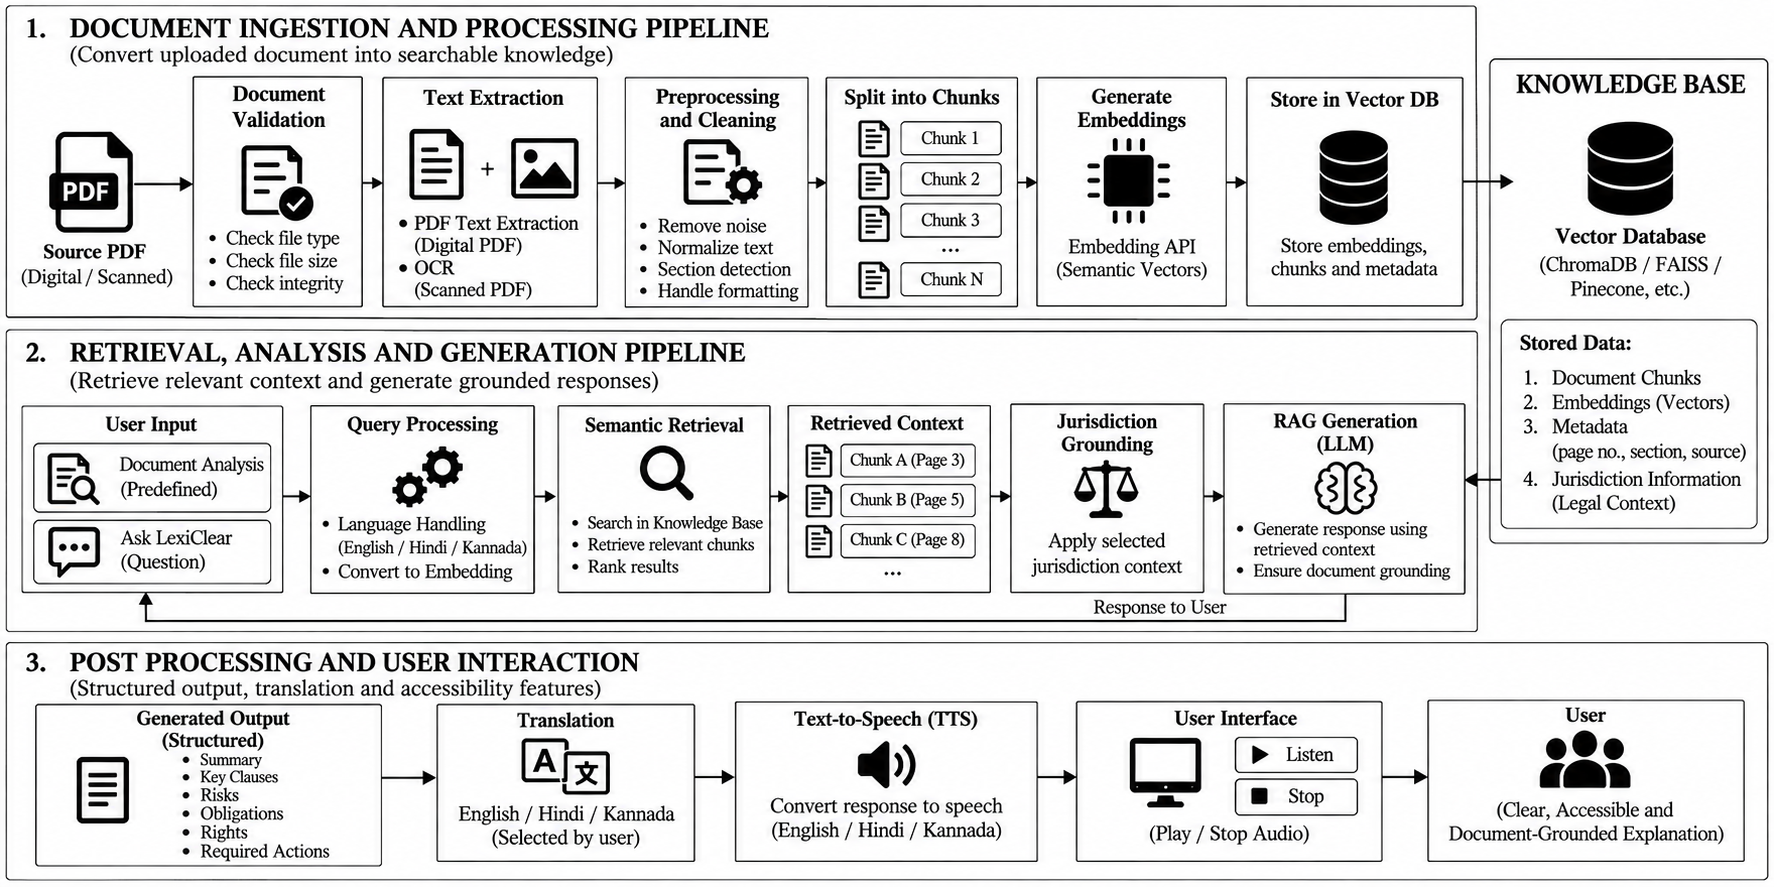
\includegraphics[width=1.0\textwidth]{img.png}
    \caption{Document Processing Pipeline of LexiClear}
    \label{fig:flowchart}
\end{figure}

Figure 3.1 describes the proposed system architecture of LexiClear and illustrates the flow of information from document upload to the delivery of an accessible, document-grounded response. The architecture is divided into three major stages: document ingestion and processing, retrieval, analysis and generation, and post processing and user interaction. Each stage performs a specific set of operations that together form the complete document-understanding workflow.

The first stage, Document Ingestion and Processing, begins with the source PDF provided by the user. The uploaded document first passes through document validation, where the file type, size, and integrity are checked. The system then performs text extraction using direct PDF text extraction for digital documents and Optical Character Recognition (OCR) for scanned or image-based PDFs. The extracted content undergoes preprocessing and cleaning to remove unwanted noise, normalize the text, identify sections, and handle formatting. The processed text is then divided into smaller chunks to make the document suitable for efficient retrieval. Each chunk is converted into a semantic vector using an embedding API. These embeddings, along with the document chunks and associated metadata, are stored in a vector database, forming the knowledge base used during subsequent retrieval operations.

The second stage, Retrieval, Analysis and Generation, handles both predefined document analysis and questions submitted through Ask LexiClear. The user's input is processed according to the selected language, and the query is converted into an embedding representation. Semantic retrieval is then performed against the knowledge base to identify and rank the most relevant document chunks. The retrieved context is passed to the jurisdiction grounding component, where the selected jurisdictional context is incorporated into the analysis. The resulting contextual information is provided to the Retrieval-Augmented Generation (RAG) component, which uses the retrieved document content and jurisdictional context to generate a grounded response. This approach helps maintain a connection between the generated response and the information contained in the uploaded document.

The final stage, Post Processing and User Interaction, converts the generated response into a form that is easier for the user to access and understand. The output is organized into structured categories such as summary, key clauses, risks, obligations, rights, and required actions. The response can then be translated into the selected language, including English, Hindi, or Kannada. The translated or generated response can also be processed through the text-to-speech component to provide audio output. The user interface provides Listen and Stop controls for audio playback. Through these stages, LexiClear provides a document-grounded explanation through multiple interaction and accessibility modes.

\chapter{Results}

The development of LexiClear resulted in an integrated prototype for processing legal and administrative documents and presenting their information in an accessible form. The implemented workflow combines document ingestion, text extraction, OCR support, semantic retrieval, Retrieval-Augmented Generation, jurisdiction grounding, structured analysis, multilingual translation, and text-to-speech functionality. The system was tested through backend and frontend integration to verify the operation of the major components.

The results presented in this chapter focus primarily on the functional behavior of the developed system. Since a large expert-labelled dataset and controlled quantitative evaluation have not yet been established, the results are described in terms of available document inputs, experimental setup, and functional observations rather than numerical accuracy or performance metrics.

\section{Dataset}

LexiClear is designed to process legal and administrative PDF documents rather than depending on a single fixed dataset. During development and functional evaluation, three legal documents were used to represent different document-understanding scenarios: an employment-related document, a Simple Mortgage Deed, and a Leave and License Agreement. These documents contain clauses, conditions, obligations, rights, responsibilities, financial terms, restrictions, and other information relevant to document-based question answering.

For evaluating the Ask LexiClear functionality, question-answer datasets were prepared in CSV format from the documents used during testing. Each CSV file contains two fields: \texttt{question} and \texttt{expected\_answer}. The questions are designed to test whether the system can retrieve and provide information corresponding to specific clauses and details present in the source document.

The first dataset,\texttt{qa\_test.csv},contains 20 question-answer pairs based on employment-related legal document.The second dataset, \texttt{mortgage\_deed\_qa\_test.csv}, contains 20 question-answer pairs based on the Simple Mortgage Deed. The third dataset, \newline \texttt{leave\_license\_agreement\_qa\_test.csv}, contains 20 question-answer pairs based on the Leave and License Agreement. Together, these datasets provide 60 document-specific question-answer pairs for functional evaluation of the document-question-answering workflow.

The document-processing pipeline supports both digital PDFs and scanned or image-based PDFs. For digital documents, text can be extracted directly from the PDF, while OCR is used when the document contains scanned or image-based content. The extracted information is subsequently divided into chunks and represented using semantic embeddings. The processed document chunks and their associated metadata form the searchable knowledge representation used by the retrieval system. Metadata can include information such as the source document, page number, section, and other available document-location details.

The QA datasets are therefore used as functional evaluation data rather than as a formally curated legal benchmark. The expected answers represent information extracted from the corresponding source documents and are used to compare the responses generated by LexiClear during testing. The datasets do not constitute expert-annotated ground truth for legal interpretation. Consequently, the evaluation is focused on functional document-based question answering rather than claims of legal accuracy, and metrics such as classification accuracy, precision, recall, or F1-score are not used unless a formal expert-annotated evaluation dataset is established.
\section{Experimental setup}
The experimental setup consists of the major software components required to implement and test the LexiClear workflow. The system follows a client-server architecture in which the frontend provides the user interface and communicates with the backend through defined endpoints.

The frontend is implemented using React with Vite. It provides interfaces for uploading documents, viewing document analysis, interacting with Ask LexiClear, selecting supported languages, and controlling speech playback through Listen and Stop controls.

The backend is implemented using FastAPI. It manages document upload, text processing, analysis requests, question answering, translation-related operations, and speech-generation requests. The backend also connects the document-processing and retrieval components required for generating document-grounded responses.

The experimental workflow begins with uploading a legal or administrative PDF. The document is validated and its textual content is extracted either through direct PDF extraction or OCR. The extracted content is preprocessed, divided into chunks, and converted into semantic embeddings. These representations are stored together with document information so that relevant content can be retrieved when an analysis request or user question is submitted.

For a user question, the query is processed and converted into a semantic representation. Relevant document chunks are retrieved from the knowledge base and passed to the RAG generation component. Jurisdiction information can also be incorporated into the generation workflow. The resulting response is then structured and can be translated into English, Hindi, or Kannada. When speech output is requested, the response is passed to the text-to-speech component.

Development and integration testing were performed in a macOS environment. The backend document-analysis endpoint was tested using a rental agreement and successfully returned structured analysis for the document content. The frontend was connected to the document upload, analysis, Ask LexiClear, and speech-related interactions.

The Kannada text-to-speech functionality was also tested during development. The system successfully generated a WAV audio file from a generated legal statement using the available Apple MPS device configuration. This verifies the functional connection between generated text and the speech-generation component.

\begin{table}[h]
\centering
\caption{Functional Verification Scenarios}
\label{tab:functional_verification}

\vspace{0.15cm}

\renewcommand{\arraystretch}{1.5}

\begin{tabular}{|p{1.2cm}|p{4.0cm}|p{7.8cm}|}
\hline
\textbf{Test ID} & \textbf{Test Scenario} & \textbf{Observed Behaviour} \\
\hline

T1 & Upload legal PDF &
The backend accepts the document for processing. \\
\hline

T2 & Process document &
Text is extracted through direct extraction or OCR depending on document type. \\
\hline

T3 & Analyze rental agreement &
Structured analysis is returned for the document content. \\
\hline

T4 & Ask document-specific question &
The question is processed through retrieval and response generation. \\
\hline

T5 & Select English, Hindi or Kannada &
The selected language is passed to the language-processing workflow. \\
\hline

T6 & Generate Kannada speech &
Kannada WAV audio is successfully generated during development testing. \\
\hline

T7 & Listen / Stop &
The frontend provides controls for starting and stopping generated audio. \\
\hline

T8 & Jurisdiction grounding &
Selected jurisdictional context is incorporated into the response-generation workflow. \\
\hline

\end{tabular}
\end{table}

The functional observations indicate that the major components of the system are integrated and can operate as a connected workflow. However, these observations represent functional verification and should not be interpreted as a formal quantitative performance evaluation.

\section{Results and Discussions}

The developed LexiClear system was evaluated through functional testing of its major components and their integration into the complete document-understanding workflow. The evaluation focused on verifying whether the system could accept legal documents, process their contents, retrieve relevant information, generate document-grounded responses, and provide multilingual and speech-based accessibility features. The results indicate that the major components of the proposed system have been successfully integrated and can operate as a connected workflow.

\subsection{Document Processing Results}
The document ingestion workflow was tested using legal PDF documents, including a rental agreement. The system successfully accepted the document through the upload interface and passed it to the backend for processing. The document-processing pipeline supports extraction of text from digital PDFs and provides OCR processing for scanned or image-based documents.

After extraction, the document content is preprocessed and divided into smaller chunks. These chunks are converted into semantic embeddings and stored along with relevant metadata for subsequent retrieval. This process establishes the searchable knowledge representation required by the retrieval and RAG components.

The functional result demonstrates that LexiClear can convert an uploaded legal document into a form that can be processed and searched semantically rather than requiring the user to manually locate relevant clauses.

\begin{figure}[h]
    \centering
    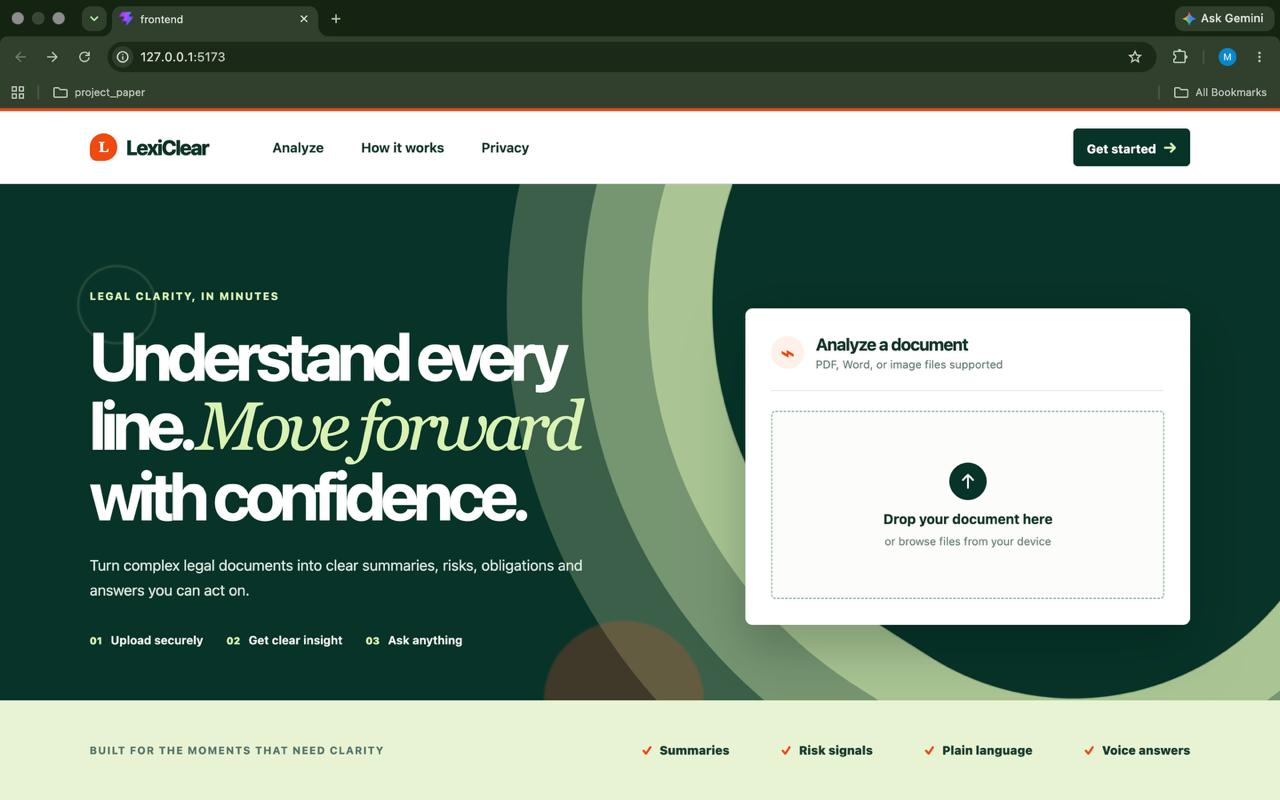
\includegraphics[width=\textwidth]{lexiclear_homepage.jpg}
    \caption{LexiClear User Interface for Document Analysis}
    \label{fig:lexiclear_interface}
\end{figure}

Figure~\ref{fig:lexiclear_interface} describes the implemented LexiClear user interface for document analysis. The interface provides the entry point for uploading supported documents and accessing the system's analysis workflow. It also presents the major accessibility-oriented capabilities of the system, including summaries, risk signals, plain-language explanations, and voice-based responses.


\subsection{Document Analysis Results}
The document-analysis functionality was tested using a rental agreement. The backend analysis endpoint successfully returned structured information from the document. The generated output organizes relevant information into categories such as summary, key clauses, risks, obligations, rights, and required actions, where applicable.

This structured representation provides a more organized alternative to presenting the user with the complete original document. It allows important information to be accessed according to its type and reduces the need to manually examine every section of a lengthy document.

However, the generated analysis should be considered an information-access and comprehension aid. The system does not independently establish the legal validity or authoritative interpretation of the identified provisions.

\subsection{Retrieval and RAG Results}
The retrieval workflow was integrated with the document-analysis and Ask LexiClear functionalities. When a user submits a question, the system processes the query and retrieves relevant document chunks from the knowledge base. The retrieved context is then supplied to the RAG generation component to produce the response.

The integration of semantic retrieval with RAG allows the generated response to be based on information retrieved from the uploaded document. This is particularly useful when the terminology used in a user's question differs from the exact wording in the document.

The result demonstrates the functional integration of the retrieval and generation stages. However, a formal evaluation using an expert-labelled question-answer dataset has not been conducted. Therefore, numerical measures such as retrieval accuracy, precision, recall, or answer-generation accuracy are not reported.

\subsection{Question-Answer Evaluation Results}

The Ask LexiClear functionality was evaluated using document-specific question-answer datasets prepared from the legal documents used during functional testing. Three CSV datasets were created for this evaluation, with each dataset containing a question and its corresponding expected answer. The datasets cover an employment-related document, a Simple Mortgage Deed, and a Leave and License Agreement.

The employment-related QA dataset contains 20 question-answer pairs, while the Simple Mortgage Deed and Leave and License Agreement datasets contain 20 question-answer pairs each. Therefore, a total of 60 document-specific questions were prepared for evaluating the question-answering workflow. The questions cover information such as obligations, rights, financial terms, conditions, restrictions, termination provisions, and other document-specific details.

During testing, each question can be submitted through the Ask LexiClear interface after the corresponding document has been processed. The system retrieves relevant document chunks and uses the retrieved context during response generation. The generated response can then be compared with the corresponding expected answer in the QA dataset to determine whether the required information has been retrieved and presented appropriately.

The QA datasets provide a structured method for functional evaluation of document-grounded question answering. They also allow different types of legal documents to be tested using questions derived from their actual contents rather than using unrelated general-purpose questions. This helps verify the integration between document processing, semantic retrieval, and RAG-based response generation.




\subsection{Jurisdiction Grounding Results}
The jurisdiction grounding component was integrated into the response-generation workflow. The selected jurisdictional context can be passed along with the retrieved document information before the response is generated.

This provides an additional contextual layer for explanations involving legal or administrative information that may vary according to jurisdiction. The jurisdiction information is used to guide the response rather than being treated as a replacement for the source document.

The effectiveness of jurisdiction grounding depends on the configured jurisdictional information and available supporting sources. Therefore, the current functional result demonstrates integration of the feature rather than a quantitative evaluation of jurisdiction-specific legal accuracy.

\subsection{Multilingual Output Results}
LexiClear provides multilingual output in English, Hindi, and Kannada. The generated response can be processed according to the language selected by the user.

The multilingual functionality extends the accessibility of the system beyond English-only interaction and allows information extracted from formal documents to be presented in languages familiar to a wider range of users. The translation workflow operates on the generated response while the original document remains the primary source of document-specific information.

No controlled translation benchmark or expert linguistic evaluation was conducted during the available testing. Consequently, the results establish functional multilingual support but do not claim a numerical translation-quality score.

\subsection{Text-to-Speech Results}
The text-to-speech component was tested as part of the accessibility workflow. During development testing, the system successfully generated a WAV audio file for Kannada text using the available Apple MPS device configuration.

The frontend also provides Listen and Stop controls for interacting with the generated audio. This establishes a connection between the generated textual response and the speech-output interface.

The speech functionality provides an alternative method of accessing generated information, particularly for users who may prefer listening to the explanation rather than reading the complete response. Further evaluation across all supported languages and different types of legal terminology would be required for a comprehensive assessment of speech quality.
\subsection{Overall Discussion}
The functional testing demonstrates that the major components of LexiClear have been connected into an end-to-end workflow. The system can accept a legal PDF, process its contents, create a retrievable document representation, retrieve relevant context, generate structured document-grounded information, answer document-specific questions, incorporate jurisdictional context, provide multilingual output, and generate speech output.

The results also indicate that the accessibility features are integrated with the core document-analysis workflow rather than operating as independent components. Translation and text-to-speech are applied to generated responses, allowing the same document-grounded information to be presented through different interaction modes.

At the same time, the current evaluation has limitations. A large expert-annotated dataset, controlled benchmark experiments, and systematic evaluation of retrieval, generation, translation, and speech quality have not yet been completed. Therefore, the results presented here are functional and integration-based results rather than statistical performance results. Future evaluation can strengthen the system assessment by using expert-annotated legal documents, predefined test questions, source-grounding measurements, multilingual evaluation, and user-based usability studies.



\chapter{Conclusion}

LexiClear was developed as an AI-assisted legal and administrative document-understanding system aimed at making complex formal documents easier for non-expert users to access and understand. The system combines document processing, semantic retrieval, Retrieval-Augmented Generation (RAG), jurisdiction grounding, structured analysis, multilingual translation, and text-to-speech within a single workflow. This integration addresses the difficulty users may face when locating and understanding important information such as clauses, obligations, rights, risks, and required actions in lengthy legal and administrative documents.


The system also incorporates jurisdiction grounding to provide additional contextual information during response generation. The structured analysis functionality organizes generated information into categories such as summary, key clauses, risks, obligations, rights, and required actions. Through the Ask LexiClear facility, users can further interact with the processed document by submitting specific questions and obtaining document-grounded responses.

Accessibility is further supported through multilingual output in English, Hindi, and Kannada, along with text-to-speech functionality. The integration of translation and speech output provides users with alternative ways of accessing generated information. Functional testing demonstrated successful integration of the major components, including document analysis of a rental agreement, frontend interaction with upload and question-answering features, and generation of Kannada speech output.

The project also has limitations that should be considered when interpreting the results. The available testing does not constitute a large-scale quantitative evaluation, and an expert-annotated benchmark dataset has not yet been established. Therefore, the system's performance cannot be represented through formal accuracy, precision, recall, translation-quality, or similar statistical measures at this stage. In addition, jurisdiction grounding and generated explanations depend on the quality and availability of the configured contextual information.

Overall, LexiClear demonstrates the feasibility of combining document processing, semantic retrieval, RAG, contextual grounding, multilingual processing, and speech-based interaction to improve access to complex legal and administrative information. The system is intended as a document comprehension and information-access aid, rather than a replacement for qualified legal advice or authoritative legal interpretation. Future development can focus on stronger source and clause-level traceability, broader jurisdiction-specific resources, additional Indian languages, voice-based input, document comparison, expert-annotated evaluation datasets, and more comprehensive usability and performance testing.
\bibliographystyle{unsrt} 
\bibliography{ref}  
\end{document}
